\chapter{Life Cycle Assessment} 
\setlength{\parindent}{15pt}
\label{ch:susdevlca}

Sustainability is an import aspect of a design, as its principle of using minimal amount of material and energy is beneficial economically. This chapter elaborates on how sustainable development is incorporated in the design, followed by its LCA to see environmental impacts of the Hybrid UAV. 

\section{Sustainable Development}

Sustainability was mainly considered as a trade-off criterion in the midterm phase, however, its impact on design choices in the final phase is minimal due to high performance requirements as well as VTOL capabilities. 

%not sure about this, we really didn't give a shit about the sustainability. could someone have a look and add some to this?


\section{Life Cycle Assessment}

The technical framework for LCA can be seen in \autoref{fig:lcatriangle}. It starts with the central block, `Goal and Scope', then flows into Impact Assessment, Improvement Assessment and Inventory Analysis \cite{lca}.

\begin{figure}[H]
    \centering
    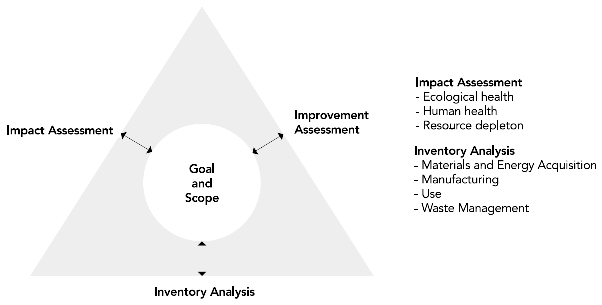
\includegraphics[width=0.8\textwidth]{LifeCycleAssessment/Figures/LCAtriangle.pdf}
    \caption{Technical Framework for Life Cycle Assessment}
    \label{fig:lcatriangle}
\end{figure}

\subsection{Goal and Scope}
The goal and scope definitions need to be determined as a first process of a LCA. The following paragraphs elaborate on details of each aspect of the first process. 

\paragraph{Goal} The MNS can be used to define the goal. The MNS states, `Carry out both supervised and autonomous monitoring and transport missions, comprising vertical take-off and landing, and high-velocity in horizontal flight.' %is this correct?

\paragraph{Scope} In order to define the assessment methods, a system to be studied and system boundaries need to be determined. Functions of the system have been identified based on a functional breakdown structure in the baseline report \cite{baseline}, and can be summarised into three categories as following: 

\begin{itemize}
    \item Perform air transport
    \item Perform various missions
    \item Perform missions under various conditions
\end{itemize}

\paragraph{Functional Unit}
A main purpose for a functional unit is to set a normalised basis of comparison. For a consistent analysis, it is decided that further quantitative comparison will have a normalised scale from 0 to 100.

\paragraph{System Boundaries}
System boundaries are defined based on requirements, which can be found in \autoref{ch:syst_desc}.

\paragraph{Data Quality}
Data quality in LCA is reflected in the final LCA. At this point of the stage, it is not possible to come up with a consistent and traceable data quality, such as time-related coverage, geographical coverage and technological coverage \cite{lca}. It will be established in the next phase of the project. 

\paragraph{Critical Review Process}
Critical review process is not applicable, since the process is mainly for certification of a system or product and publication of the project in terms of environmental standards.

\subsection{Inventory Analysis} 
Inventory analysis is carried out after defining goal and scope definition. The online U.S Life Cycle Inventory Database\footnote{\url{https://uslci.lcacommons.gov/uslci/search}} and the offline version \cite{USLCI} are used to determine specifications of 3 different phases that are shown in \autoref{fig:lcawheel} as following: product manufacturing, use, end of life. The analysed items adhere to the production plan, which can be found in \autoref{ch:prod_plan}. Each Life Cycle Inventory (LCI) data is directly taken from the U.S Life Cycle Inventory Database. The inventory analysis primarily uses $CO_{2}$ footprint and Cumulative Energy Demand (CED).

\nomenclature[A]{CED}{Cumulative Energy Demand}

\paragraph{Assumptions} There are several assumptions used for LCI.
\begin{itemize}
    \item For E-glass composites, the ratio of E-glass and high density polyethylene resin is 1:1.
    \item Carbon fibre composites are mainly made from acrylonitrile copolymer.
    \item Possible choices for different production methods are eliminated and assume that environmental impacts of all manufactured components do not differ in terms of different production methods.
    \item Batteries are recharged by a natural gas powerplant in the Netherlands.
\end{itemize}

\nomenclature{LCI}{Life Cycle Inventory}

\begin{figure}[H]
    \centering
    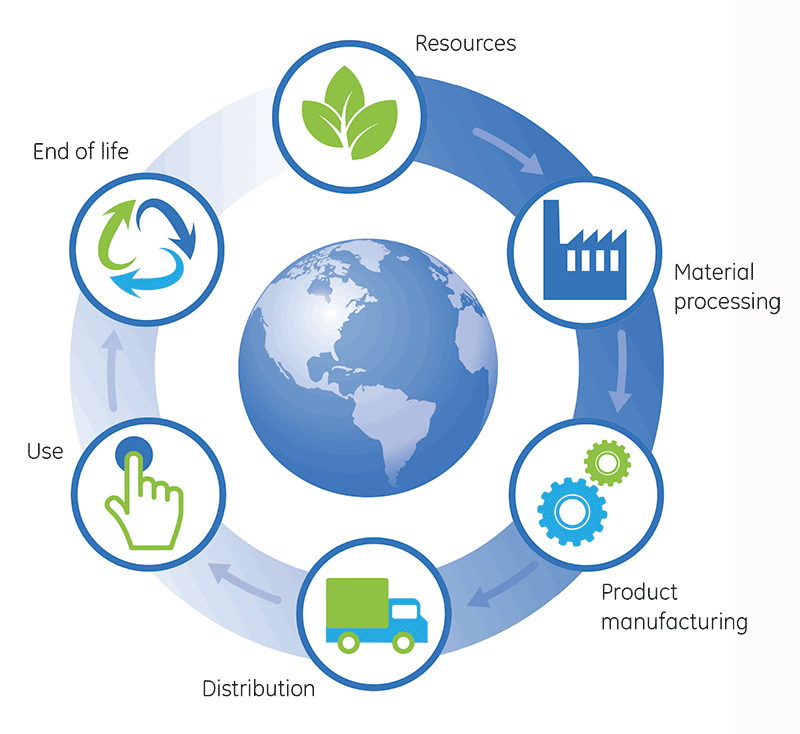
\includegraphics[width=0.5\textwidth]{LifeCycleAssessment/Figures/lcadiagram.jpg}
    \caption{Life Cycle Assessment Wheel}
    \label{fig:lcawheel}
\end{figure}

\paragraph{Materials \& Energy Acquisition and Manufacturing Phase} This section analyses $CO_{2}$ footprint and CED for manufactured components, as purchased components are not considered for materials \& energy acquisition and manufacturing phase.\\
For the fuselage, E-glass and high density polyethylene resin are used. To produce the fuselage, 3.633 kg of $CO_{2}$ is emitted and 201.9 MJ of CED is needed, which can be seen in \autoref{tab:eglasscomp}

\begin{table}[H]
\centering
\caption{Fuselage Production LCI}
\label{tab:eglasscomp}
    \begin{tabular}{lcc}
    \toprule
    Material per kilogram         &$ CO_{2}$ footprint [kg] & CED [MJ]  \\\midrule
    E-glass                         & 0.141                & 4.572    \\\hdashline
    High density polyethylene resin & 1.312                & 76.20    \\\hline \hline
    \textbf{Fuselage total (2.5 kg)}                 & \textbf{3.633}                & \textbf{201.9}   \\\bottomrule
    \end{tabular}
\end{table}

A carbon fibre rod and Expanded Polypropylene (EPP) foam are used to produce the wing. Most carbon fibre composites are made from polyacrylonitrile as their base\footnote{\url{http://www.compositesworld.com/blog/post/the-making-of-carbon-fiber}, Acessed on 26-06-2017}. The LCI of the wing can be seen in \autoref{tab:winglci}. In order to produce the wing, 5.642 kg of $CO_{2}$ is emitted and 217.8 MJ of CED is needed.

\nomenclature[A]{EPP}{Expanded Polypropylene}

\begin{table}[H]
\centering
\caption{Wing Production LCI}
\label{tab:winglci}
    \begin{tabular}{lcc}
    \toprule
    Material per kilogram       & $CO_{2}$ footprint [kg] & CED [MJ] \\\midrule
    Acrylonitrile copolymer     & 3.134                & 105.3    \\\hdashline
    Polypropylene resin for EPP & 1.216                & 75.20    \\\hline
    Carbon fibre rod (0.588 kg)       &  1.843                    &  61.92        \\\hdashline
    Carbon fibre ribs (0.893 kg)      &   2.799                  &  94.03           \\\hdashline
    EPP foam (0.822 kg)         &   1.000                   &  61.81        \\\hline \hline
    \textbf{Wing total (2.500 kg)}   & \textbf{5.646}                     & \textbf{217.8}              \\\bottomrule
    \end{tabular}
\end{table}

For painting the UAV, a method of simple top coat is chosen. Per square meter of surface area, 0.731 kg of $CO_{2}$ is emitted and CED of  10.24 MJ is required. The total surface area of the UAV and corresponding $CO_{2}$ \& CED values can be seen in \autoref{tab:painting}. The surface area of the wing, the horizontal stabiliser and the vertical tail are multiplied by 2, as both sides of each component have to be painted. 3.056 kg of $CO_{2}$ is emitted and 31.29 MJ of CED is required in order to paint the UAV.

\begin{table}[H]
\centering
\caption{UAV Painting LCI}
\label{tab:painting}
    \begin{tabular}{lccc}
    \toprule
                          & Surface area [$m^2$] & $CO_{2}$ footprint [kg] & CED [MJ] \\\midrule
    Automotive painting (top coat) & 1  &   0.7310 & 10.24 \\\hline
    Fuselage              & 1.184                    & 0.8655                 & 12.12    \\\hdashline
    Wing                  & $0.8010\cdot2$                 & 1.171                  & 16.40    \\\hdashline
    Horizontal stabiliser & $0.1062\cdot2$                 & 0.1553                 & 2.175    \\\hdashline
    Vertical tail         & $0.02893\cdot2$                & 0.04230                & 0.5925   \\\hline \hline
    \textbf{UAV total}             & \textbf{3.056}                    & \textbf{2.234}                  & \textbf{31.29}    \\\bottomrule
    \end{tabular}
\end{table}

For transporting manufactured parts, a diesel-powered combination truck is used. Per km of transport, the truck emits 0.0799 kg of $CO_{2}$. However, distance between a factory and an assembly facility is not defined, thus the transport $CO_{2}$ footprint will not be considered for analysis.

\paragraph{Use Phase}
%something about transport and battery-charging
During the use phase, batteries have to be charged per mission. Per GJ of heat generated by a natural gas powerplant, it emits 56 kg of $CO_{2}$\cite{USLCI}. In order to transfer the heat to electricity, an efficiency of 39 \% is taken \cite{electricity}. Thus, 56 kg of $CO_{2}$ is emitted from generating 0.39 GJ of electricity. Using the battery capacity of 24190 mAh as the most extreme flight scenario, required power can be found to be 467 W, based on \autoref{eq:battcap} and P = I*V. Defining that the flight time for the most extreme flight scenario is 115 minutes according to \autoref{tab:extreme}. By multiplying the required power with time, which is $467\cdot115\cdot60$, the required energy is 3.222 MJ per the most extreme flight scenario mission. The requirement SYS-OP-2.1 states that the UAV shall have an operational life of at least 1500 flying hours. By dividing 1500 flying hours with 115 minutes of each mission, 783 missions can be launched. Thus, $3.222\cdot783$ MJ of energy is needed to recharge batteries for 783 missions, which translates to 2.523 GJ of electricity. By dividing the required electricity with the unit electricity of 0.39 GJ and multiplying it by the unit $CO_{2}$ footprint of 56 kg, 362.3 kg of $CO_{2}$ is emitted for 1500 flying hours. 

\paragraph{Waste Management}
EPP can be fully recycled into new wing parts, while carbon fibre rods and ribs cannot be recycled into new parts due to undesirable reduction in mechanical properties. Thus, the carbon fibre parts are considered as waste to be left in deposit containers at collection points. $CO_{2}$ footprint of the disposal method is 0.040 kg and CED of 0.55 MJ is required.\\
Disposal of lipo batteries is landfill safe, if they are processed with a salt water method, which discharges the batteries slowly and completely as well as neutralises the lithium. Thus, no carbon footprint and CED are considered for disposing lipo batteries.\\
Raw materials such as gold, silver, palladium and platinum are first extracted from circuit boards then metal parts such as steel and aluminium are removed. Then the plain circuit boards are chopped and recycled into different products or new circuit boards. Thus, no carbon footprint and CED are considered here.

\subsection{Impact Analysis}
Impact analysis is left for future as data regarding the following cannot be found without a proper license to access to detailed online database: abiotic resources, biotic resources, land use, global warming, stratospheric ozone depletion, ecotoxicological impacts, human toxicological impacts, photochemical oxidant formation, acidifitcation, eutrophication and work environment.


\subsection{Interpretation}
With the complete inventory analysis, it is possible to identity hot-spots of the UAV in terms of $CO_{2}$ footprint and CED. \autoref{tab:hotspot} shows carbon footprint and CED for different elements analysed for LCI. Recharging batteries for 1500 flight hours emits the most $CO_{2}$ of 362.3 kg and requires the highest CED of 2523 MJ. Thus, recharging batteries during the use phase is the hot-spot.


\begin{table}[H]
\centering
\caption{Hot-Spot Identification for LCI}
    \label{tab:hotspot}
    \begin{tabular}{l|cc}
    \toprule
                                           & $CO_{2}$ emission [kg]        & CED [MJ]                     \\\hdashline
    Fuselage production                    & 3.633                         & 201.9                        \\\hdashline
    Wing production                        & 5.646                         & 217.8                        \\\hdashline
    UAV painting                           & 2.234                         & 31.29                        \\\hdashline
    Battery recharge (1500 flight hours) & \cellcolor[HTML]{FE0000}362.3 & \cellcolor[HTML]{FE0000}2523 \\\hdashline
    Part disposal                          & 0.040                         & 0.550   \\\bottomrule                    
    \end{tabular}
\end{table}

As a recommendation, different types of propulsion systems should be considered for future, such as a hybrid propulsion, an internal combustion propulsion or electric propulsion powered by renewable energy. 



